\documentclass[fr]{../../../../../../eplexam}
\usepackage{../../../../../../eplunits}
\usepackage{circuitikz}
\usepackage{pgfplots}
\usepackage{enumitem}
\pgfplotsset{compat=newest}
\tikzset{meter/.style={draw,thick,circle,fill=white,minimum size =0.75cm,inner sep=0pt}}

\hypertitle{circmes-ELEC1370}{4}{ELEC}{1370}{2014}{Juin}{Majeure}
{Nicolas Verbeek\and Adrien Couplet\and Martin Van Essche\and Guillaume Gilson\and Guillaume Colinet}
{Claude Oestges, Bruno Dehez and Christophe Craeye}

\section{Question Oestges : phaseurs}
On considère le circuit suivant
\begin{center}
    \begin{circuitikz} 
    	\draw
		to[american voltage source,l=$12\angle\ang{0}$] (0,2.5) 
  		(2.5,2.5) to[R,l=$\SI{2}{\ohm}$] (0,2.5)
  		(2.5,2.5) to [C,l=-j$\SI{1}{\ohm}$] (5,2.5)
  		(2.5,0) to[european resistor,l=$Z$,-*] (2.5,2.5)
 		(5,2.5) to[R,v=$V_o$,l=$\SI{1}{\ohm}$] (5,0)
 		(0,0) -- (5,0);
 	\end{circuitikz}
\end{center}
On mesure une tension $V_o=3\angle\ang{20}$V. On demande de calculer
\begin{enumerate}
    \item La valeur de l'impédance $Z$
    \item La valeur de l'inductance ou capacité mise en série avec une résistance de l'impédance $Z$
    \item La puissance active et la puissance réactive fournie par la source
    \item La valeur de $Z = R + Xj$ (avec $R>0$) pour que la puissance réactive fournie par la source soit nulle
\end{enumerate}

\begin{solution}
Solutions finales (contrôlées avec LTSpice):
\begin{enumerate}
    \item $Z = 3.35\angle\ang{-19.12} = 3.165 - 1.097j$
    \item La partie imaginaire est négative, il s'agit d'une capacité
    \[ C = \frac{1}{1.097\omega} \]
    \item La puissance complexe vaut $S = 25.02 \angle\ang{-12.4} = 24.4 - 5.37j$.\\ Donc $P=\SI{24.4}{\watt}$ et $Q=5.37$ VAR.
    \item Il faut que la puissance complexe soit purement réelle, et donc on trouve (par exemple) que $Z=1+j$.
\end{enumerate}
\end{solution}

\section{Question Oestges : Bode et quadripôles}
On considère le circuit suivant
\begin{center}
	\begin{circuitikz}
		\draw
		(0,1) node [above]{$V_\text{in}$} to [short,o-] (1,1) 
		 to [C,l=$C_1$,*-] (4,1)
		(1,1) -- (1,2.5) to [R,l=$R_2$] (4,2.5) -- (4,1) to [C,l=$C_2$] (4,-3)
		(8,0.5) node[op amp, yscale=-1] (opamp) {}
		(opamp.-) -- (5.5,0) -- (5.5,-1.2) to [R,l=$R_4$,*-] (10,-1.2) -- (10,0.5)
		(5.5,-1.2) to [R,l=$R_3$] (5.5,-3)
		(opamp.+) to [short,-*] (4,1)
		(opamp.out) -- (10,0.5) to [short,*-o] (11,0.5) node [above]{$V_\text{out}$}
		(-1,-3) -- (11,-3);
	\end{circuitikz}
\end{center}
On demande de calculer
\begin{enumerate}
    \item La matrice $G$ associée au quadripôle de ce circuit
    \item Tracer le diagramme de Bode (amplitude et phase) du coefficient $g_f$ et en déduire la fonction de ce circuit.
    \item Déterminer $Z_\text{out}$ si $Z_\text{in} = \SI{100}{\ohm}$.
\end{enumerate}
PS: il manque les données pour tracer le diagramme de Bode correctement

\begin{solution}
	\begin{enumerate}
    \item On obtient les coefficients $g_{r}$ et $g_{o}$ de la matrice G du quadripôle en fermant l'entrée ($V_{i} = 0$) et en plaçant une source de courant test à la sortie. Les coefficients $g_{i}$ et $g_{f} $ s'obtiennent en laissant la sortie ouverte ($i_{0}$ = 0) et en plaçant une source test de tension à l'entrée. \\
    $g_{r} = \frac{i_{i}}{i_{o}}$: on voit que le courant provenant de la source test placée en sortie va entièrement rentré dans l'ampli-op car son impédance de sortie est supposée nulle. Ainsi, les tensions aux bornes + et - de l'amplificateur sont nulles et $i_{i} = 0$\\
    $g_{r} = 0$ \\
    $g_{o}$: même raisonnement que pour $g_{r}$. La tension en sortie du quadripôle est nulle et par conséquent $g_{o} = 0$ \\
    $g_{i} = \frac{i_{i}}{v_{i}}$: en considérant qu'aucun courant ne rentre dans l'ampli-op on trouve:
    \begin{equation*}
        v_{i} = i_{i}\left(\frac{R_{2}}{1+j\omega C_{1}R_{2}} + \frac{1}{j\omega C_{2}} \right)
    \end{equation*}
    et donc
    \begin{equation*}
        g_{i} = \frac{(j\omega)^{2}C_{1}R_{2}C_{2}+j\omega C_{2}}{1+(R_{2}C_{2} + C_{1}R_{2})j\omega}
    \end{equation*}
    $g_{f} = \frac{V_{o}}{V_{i}}$: à nouveau en ne considérant qu'aucun courant ne rentre dans l'ampli-op et que les tensions aux bornes de ce dernier sont identiques on trouve:
    \begin{equation*}
        g_{f} = \left(\frac{R_{4}}{R_{3}}+1\right)\frac{1+j \omega C_{1}R_{2}}{1+j \omega(R_{2}(C_{2} + C_{1}))}
    \end{equation*} 
    \item Diagramme de Bode de $g_{f}$: en posant $\omega _{1} = \frac{1}{C_{1}R_{2}}$ et $\omega _{2} = \frac{1}{R_{2}(C_{2}+C_{1})}$, on voit que $\omega_{1} > \omega_{2}$,
    \begin{itemize}
        \item $log\left(\frac{R_{4}}{R_{3}}+1\right)$ pour $\omega <  \omega_{2}$ (pente de 0db/dec)
        \item pente de -20dB/dec pour $ \omega_{2}< \omega < \omega_{1}$
        \item pente de 0dB/dec pour $\omega > \omega_{1}$
    \end{itemize}
    \item $Z_{out}=0$ (deux façons de s'en convaincre, intuitivement l'impédance de sortie d'un ampli op idéal est nul, l'autre façon est de regarder le tableau des caractéristiques externes)
\end{enumerate}
\end{solution}

\section{Question Dehez : circuit magnétique couplé}
\begin{center}
    \begin{circuitikz}
		\draw[american currents]
		(0,0) to [american voltage source,l=$V_s$] (0,3)
  		(0,0) -- (3,0)
  		(3,3) to [R,v^=$V_x$,l_=$\SI{5}{\kilo\ohm}$] (3,0)
  		(3,3) to [R, l_=$\SI{1}{\kilo\ohm}$] (0,3)
  		(3,0) -- (6,0);
		\draw[american currents]
  		(6,3) to [cI_=$0.04V_x$] (6,0)
  		(6,0) to [short, -o] (9,0)
  		(8,0) to [R,l=$\SI{10}{\kilo\ohm}$] (8,3)
  		(9,0) to [open,v_>=$V_o$] (9,3)
  		(9,3) to [short, o-] (8,3)
  		to [short, *-] (6,3);
	\end{circuitikz}
\end{center}
On demande de
\begin{enumerate}
    \item Représenter le dipôle équivalent de Thévenin de ce circuit
    \item Supposons qu'on connecte ce circuit à un transformateur idéal avec rapport $a:1$ et une résistance de $\SI{16}{\ohm}$. Quelle valeur de $a$ maximise la puissance fournie à cette résistance?
\end{enumerate}

\begin{solution}
\begin{enumerate}
    \item $V_\text{oc} = -333.3 V_s$ et $R_\text{th} = \SI{10}{\kilo\ohm}$.
    \item On obtient un maximum de puissance pour $a=25$.
\end{enumerate}
\end{solution}

\section{Question Craeye : transitoire} 
Soit le circuit suivant dont l'interrupteur 2V s'ouvre et l'interrupteur 1V se ferme en $t=0$.
\begin{center}
    \begin{circuitikz} 
    	\draw
 		(0,0) -- (5,0)
 		(3.6,5)--(5,5) 
 		(-1.5,0) -- (0,0)
 		(-1.5,0) to[american voltage source,l=1V] (-1.5,2.5) to [closing switch,l=$t{=}0$] (-1.5,5) -- (0,5)
 		(0,0) to[american voltage source,l=2V] (0,2.5) to [opening switch,l=$t{=}0$] (0,5) to [R,l=$R_1$,*-] (1.8,5)
		(1.8,5) to [L,l=$L$] (3.6,5)
 		(5,5) to [R,l=$R_2$] (5,0)
		(6,3.6) to [open, v^=$V_o$] (6,1)
 		(3.6,5) to [C,l=$C$] (3.6,0);
 	\end{circuitikz}
\end{center}
On demande la tension $V_o$ en $t>0$ avec les données numériques suivantes : $R_1=R_2=\SI{1}{\ohm}$, $L=\SI{1}{\milli\henry}$, $C = \SI{1}{\milli\farad}$

\begin{solution}
Les conditions initiales sur le courant de l'inductance et sur la tension aux bornes de la capacité sont le suivantes:
\[ V_{L}(0-) = \SI{1}{\volt} \]
\[ I_{L}(0-) = \SI{1}{\ampere} \]
En incluant les conditions initiales, on obtient l'expression suivante pour la tension $V_{0}$ dans le domaine de Laplace:
\begin{equation*}
    V_{0}(s) = \frac{10^{-6}s^{2}+2\cdot 10^{-3}s +1}{s(10^{-6}s^{2} + 2\cdot 10^{-3}s +2)}
\end{equation*}
Qu'on peut développer en fractions simples:
\begin{equation*}
    V_{0}(s) = \frac{0.5}{s} + \frac{5 \cdot 10^{-7}s + 10^{-3}}{10^{-6}s^{2} + 2\cdot 10^{-3}s + 2}
\end{equation*}
On obtient ainsi l'expression analytique de la solution:
\[ V_o(t) = \left[\frac{1}{2} + 0.708 e^{-10^3t} \cos(10^3 t + 0.785) \right]u(t) \]

En utilisant les propriétés $ f(s)= \frac{s-b}{(s-b)^{2}+a^{2}} \rightarrow F(t) = e^{bt} cos(at)$ et $f(s) = \frac{1}{(s-b)^{2}+a^{2}} \rightarrow  F(t) = \frac{e^{bt} sin(at)}{a}$ des tables de transformées inverses de Laplace, on peut réécrire la solution sous la forme suivante:
\[V_o(t) = \left[\frac{1}{2} + \frac{1}{2}e^{-10^3t}\cos(10^3t) + \frac{1}{2}e^{-10^3t}\sin(10^3t) \right]u(t) \]

Le graphe ressemble à
\begin{center}
    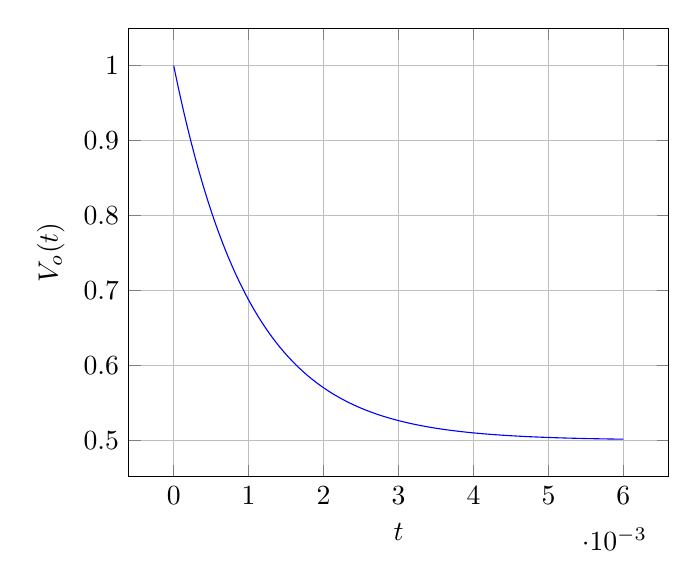
\begin{tikzpicture}
        \begin{axis}[enlargelimits=true,grid=major,ylabel=$V_o(t)$,xlabel=$t$]
            \addplot [blue,domain=0:0.006,samples=200]{(1/2)+(1/2)*e^(-10^3*x)*cos(10^3*x)+(1/2)*e^(-10^3*x)*sin(10^3*x)};
        \end{axis}
    \end{tikzpicture}
\end{center}

\end{solution}

\end{document}
